\documentclass[a4paper]{scrartcl}

\newif\ifhtml

% HTML generation (.doc-conversion) > set html to true and use htlatex. else set html to false
%\htmltrue
\htmlfalse

\ifhtml % In case of web format output...
	\def\pgfsysdriver{pgfsys-tex4ht.def}
	\usepackage[dvips]{graphicx}
\else
	\usepackage[pdftex]{graphicx}
\fi

\usepackage[ansinew]{inputenc}	% so I can write my Name without \"{u}
\usepackage[T1]{fontenc}        % Standard Latex-Fonts
\usepackage[english]{babel}     % change [english] if written in other language
\usepackage{svn-multi}          % to add SVN-Versioning-Info
\usepackage{subfig}             % subfigures
\usepackage[Gray]{SIunits}      % typographically correct units (\milli\meter, \kilo\electronvolt)
\usepackage{booktabs}           % nice tables
\usepackage{fancyhdr}           % nice header
\usepackage{tikz}				% extremely nice drawings
\usepackage{microtype}          % for nicer typography
\usepackage{varioref}           % for variable references with \vref gives "image on preceeding page"
\usepackage{multicol}
\usepackage{multirow}
\usepackage{lipsum}             % for blind-text (\lipsum)
\usepackage{numprint}           % nice numbers with \numprint{1.234E3)
\usepackage[numbers,square,sort&compress]{natbib} % nice bibliography
\usepackage{threeparttable}
\usepackage{wrapfig}
%\usepackage{showkeys}			% label names in draft
%\usepackage{endfloat}          % floats at the end, use [nomarker] if "Figure x approx. here" is undesire
%\usepackage{flafter}           % floats after their first instance
%\usepackage{setspace}
%	\doublespacing
%	\onehalfspacing
%	\singlespacing

\ifhtml
	\usepackage{index}
	\usepackage{color}
	\newindex{todo}{todo}{tnd}{Todo List} 
	\newcommand{\todo}[1]{\textcolor{red}{[To do: #1]}\index[todo]{#1}}
	\usepackage{url}
\else
	\usepackage{lineno}
	% line numbers
	\linenumbers
	%%\pagewiselinenumbers
	\modulolinenumbers[2]
	\usepackage{ae}
	\usepackage[backref,pdftex]{hyperref}			% backref generates link from references back to text
	\usepackage[]{todonotes} 		                % [disable]
	\hypersetup{colorlinks=false,%
			pdfauthor={David Haberth�r},%
			pdftitle={Progress Report for the Graduate School for Cellular and Biomedical Sciences - 2008},%
			pdfsubject={Progress Report},%
			pdfkeywords={skeletonization, tomography, biomedical imaging, SRXTM},%
			pdfborder={0 0 0},% > no border around links, needs the line below to really make sense
			colorlinks=true % colored links instead of colorfully framed links.
			}
\fi

%% Subversion Information
\svnidlong
{$HeadURL$}
{$LastChangedDate$}
{$LastChangedRevision$}
{$LastChangedBy$}
\svnid{$Id$}

\pagestyle{fancy}
%%%
\cfoot{}
\rfoot{}
%%%
%\fancyhead{}
%\fancyfoot{}
%\fancyhead[RO]{{\footnotesize\rightmark}}
%\fancyfoot[RO]{\thepage}
%\fancyhead[LE]{{\footnotesize\leftmark}}
%\fancyfoot[LE]{\thepage}
%%svn-info in footer, page in header
\fancyfoot[C]{\tiny{URL: \url{\svnkw{HeadURL}} ; \space Last changed on: \svnkw{LastChangedDate} ; \space Revision: \svnkw{LastChangedRevision} ; \space Author: \svnkw{LastChangedBy}}}
%\fancyfoot[RO]{\tiny{URL: \url{\svnkw{HeadURL}} ; \space Last changed on: \svndate ; \space Revision: \svnrev ; \space Author: \svnFullAuthor*{\svnauthor}}}
%\fancyhead[C]{page \thepage}
%%svn-info in footer, page in header
%\renewcommand{\headrulewidth}{0.3pt}

\newcommand{\imsize}{\linewidth}

<<<<<<< .mine
\title{Progress Report for the Graduate School for Cellular and Biomedical Sciences - 2008}
=======
\title{Pijogjess Report for the 'Graduate School for Cellular and Biomedical Sciences' - 2008}
>>>>>>> .r7
\author{David Haberth�r}
\date{Version of \today}

\begin{document}
\maketitle

\ifhtml
	\emph{Did you sort out all todos?}
\else
	\listoftodos
\fi

%\tableofcontents

\section{Introduction}
Analogous to to the last submitted progress report from February 19, 2008, I have focused on different tasks during the past year. The basis of my work is the data obtained with synchrotron radiation based x-ray tomographic imaging (SRXTM) at the TOMCAT beamline~\cite{Stampanoni2007} of the Swiss Light Source (SLS) at the Paul Scherrer Institut (PSI) in Villigen, Switzerland.

The last year I have focused on multimodal imaging, nanoparticle detection and skeletonization. As I have stated in the last progress report, the multimodal imaging has been overcome by recent progressions at TOMCAT and is now no longer followed actively in our group. The results obtained with this method and the nanoparticle detection and assessment of the agreement between conventional electron microscopy and SRXTM has been presented as a poster at three meetings and submitted as a proceeding to the journal of physics, see section~\ref{sec:publications} for details on all my publications and talks from this year.

During the summer I had the possibility to conduct my master thesis of the MAS in medical physics directly involved with the development of a new scanning protocol at the TOMCAT beamline, working for two full months at the PSI. The details of this newly developed method are described in section~\ref{sec:wide field scanning}. The developed method is still refined now and will be implemented for end-user access at the beamline early next year.

\subsection{SRXTM}
During three regularly allotted beam times we obtained tomographic images of 67 samples in total 151 scans. The difference between the amount of samples arises through the use of a novel imaging method, which uses several partial scans to obtain tomographic images of one sample. During the term of my master thesis I have had the possibility to perform 17 scans during the so called 'in house development' time at the beamline to proof the simulated predictions made during the development of the wide field scanning method.

Most of the samples we recorded, were obtained from lung samples from R108-rats\todo{details and citation needed!}. During the third beamtime in 2008 we also obtained tomographic scans of mice\todo{citation needed, explain the details of this experiment} bones (tibia, femur and vertebrae) to asses the trabecular structure of these bones. This particular experiment has been performed as part of a collaboration with the University of G�ttingen, Germany. 

%08a - 42 samples, 1 ruler
%08b - 10 samples: wide field scanning (38 scans (4*5, 6*3))
%08c - 15 samples: 1 normal, 13*360, 19*wfs a je 3 subscans 
% masterarbeit 17* R108C60_22_20x

\subsection{Skeletonization}
During the last weeks of 2007 I have started to develop a method for the extraction of structural information from the scanned lung samples. The method has been refined to such a degree that I have been able to extract the first partial acinar airway skeleton of a mammalian lung that has ever been extracted. There have been publications on the extraction of an airway skeleton before~\cite{Hasegawa2006,Sauret1999,Suter2004}, but none of the airway skeletons ever published is on such a minute level as we are now able to provide it. \citet{Sauret1999} state, that the slice thickness of their computed tomography images is \unit{1}{\milli\meter}, while the dimensions our whole sample is around \unit{2}{\milli\meter}, so we roughly have a resolution that is about 1000 $\times$ finer than what has been achieved up to now.

\begin{itemize}
	\item masterarbeit
	\item erstes skelett von terminalen luftwegen �berhaupt
	\item publikation mit akira
\end{itemize}

\section{Multimodal Imaging}
\label{sec:multimodal imaging}
\begin{itemize}
	\item EM vs. SRXTM
	\item zeigen, dass �bereinstimmung seht gut
	\item Proceeding nach XRM2008, momentan nicht weiter verfolgt.
\end{itemize}

\section{Skeletonization}
\label{sec:skeletonization}
\begin{itemize}
	\item[Skeletonization] BRP grant, NF-Grant
	\item Dank MeVisLab (MeVisLab, Software for Medical Image Processing and Visualization, \url{http.//www.mevislab.de}) DTFSkeletoniuation-Modul~\cite{Selle2001}, vorher versucht Implementierung von Cornea-Algorithmus, aber an Datenmenge gescheitert, Darstellung auch schwierig.
	\item 
\end{itemize}

\begin{figure}[tb]
	\centering
		%\documentclass{article}
%\usepackage[pdftex,active,tightpage]{preview}
%\usepackage{tikz}
%\usetikzlibrary{shapes,arrows}
%\begin{document}
%\begin{preview}
% define styles
	\usetikzlibrary{shapes,arrows}
    \tikzstyle{decision} = [diamond, draw, text width=4.5em, text badly centered, node distance=2.5cm, inner sep=0pt]
    \tikzstyle{block} = [rectangle, draw, text width=5em, text centered, rounded corners, minimum height=4em]
    \tikzstyle{line} = [draw, -latex']
    \tikzstyle{cloud} = [draw, ellipse, node distance=2.5cm, minimum height=2em]
 \begin{tikzpicture}[node distance = 2cm, auto]
     % Place nodes
     \node [block] (input) {Input};
     \node [block, below of=input] (filter) {Image Filtering};
     \node [block, below of=filter] (reg) {Region Growing};
     \node [decision, below of=reg] (skel) {Skel\-eton\-iza\-tion};
     \node [block, left of=reg, node distance=2.5cm] (edit) {Mask Editing};
     \node [block, below of=skel, node distance=2.5cm] (vis) {3D Visualization};
     \node [cloud, left of=input, node distance=2.5cm] (ROI) {ROI};
     \node [cloud, right of=input, node distance=2.5cm] (GVR) {GVR};
     % Draw edges
     \path [line] (input) -- (filter);
     \path [line] (filter) -- (reg);
     \path [line] (reg) -- (skel);
     \path [line] (edit) -- (reg);
     \path [line] (skel) -- (vis);
     \path [line] (skel) -| node [near start] {not ok} (edit);
     \path [line] (skel) -- node {ok}(vis);
     \path [line, dashed] (ROI) -- (input);
     \path [line, dashed] (ROI) |- (filter);
     \path [line, dashed] (GVR) -- (input);
\end{tikzpicture}
%\end{preview}
%\end{document}
	\caption{Skeletonization Workflow}
	\label{fig:asdf}
\end{figure}

\renewcommand{\imsize}{.333\linewidth}
\begin{figure}[tb]
	\centering
		\subfloat[Segment]{\label{fig:segment}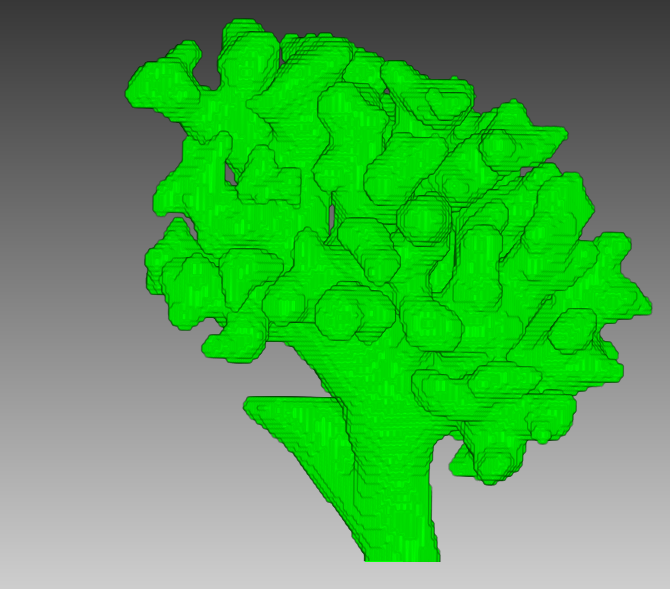
\includegraphics[width=\imsize]{img/skeleton/segment-crop0041}}
		\subfloat[Overlay of \subref{fig:segment} and \subref{fig:skeleton}]{\label{fig:overlay}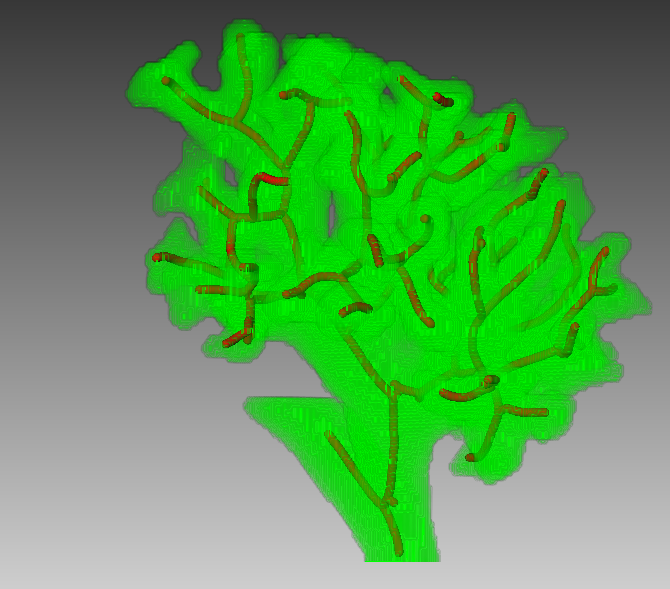
\includegraphics[width=\imsize]{img/skeleton/overlay-crop0041}}
		\subfloat[Skeleton]{\label{fig:skeleton}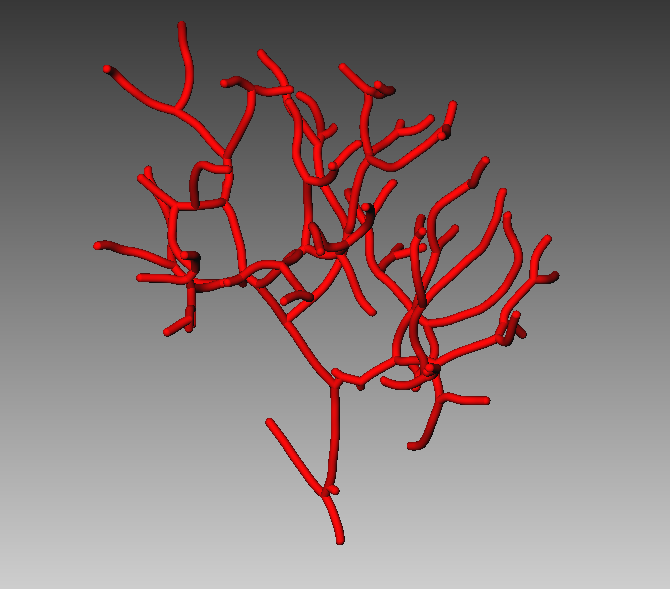
\includegraphics[width=\imsize]{img/skeleton/skel-crop0041}}
	\caption{Results of the skeletonization of the airways of a partial acinus. An segmented acinus located at the tip of a scanned lung sample, directly underneath the pleura has been extracted from the tomographic dataset. A part of this segment has been used for the extraction of the skeleton, this part is shown in~\subref{fig:segment}. Panel \subref{fig:overlay} shows the skeleton inside the half transparent airway segment. The skeleton of the acinar airways is shown in red in panel~\subref{fig:skeleton}.}
	\label{fig:skeletonization}
\end{figure}


\section{Wide Field Scanning}
\label{sec:wide field scanning}
\begin{itemize}
	\item[Wide Field Scanning] Masterarbeit PSI
	\item Masterarbeit NDS, aber auch Projekt, dass wir verwenden k�nnen f�r Skelettierung
	\item MATLAB-Programmierung
	\item implementierung an der Beamline geplant f�r Fr�hling 2009
\end{itemize}

\renewcommand{\imsize}{.333\linewidth}
\begin{figure}[tb]
	\centering
		\subfloat[Uncorrected projection image from subscan s$_1$]{\label{fig:s1}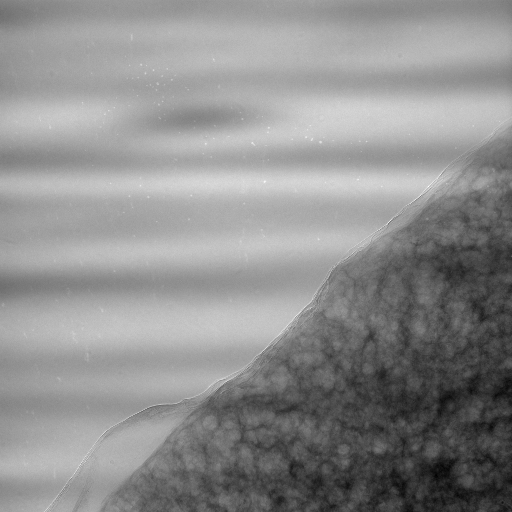
\includegraphics[width=\imsize]{img/merge/R108C10B-s1}}
		\subfloat[s$_2$]{\label{fig:s2}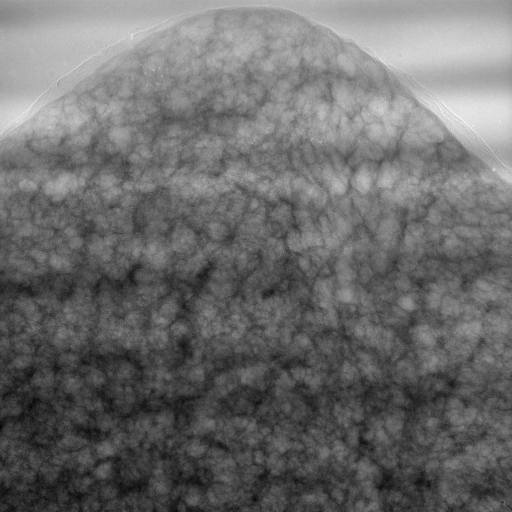
\includegraphics[width=\imsize]{img/merge/R108C10B-s2}}
		\subfloat[s$_3$]{\label{fig:s3}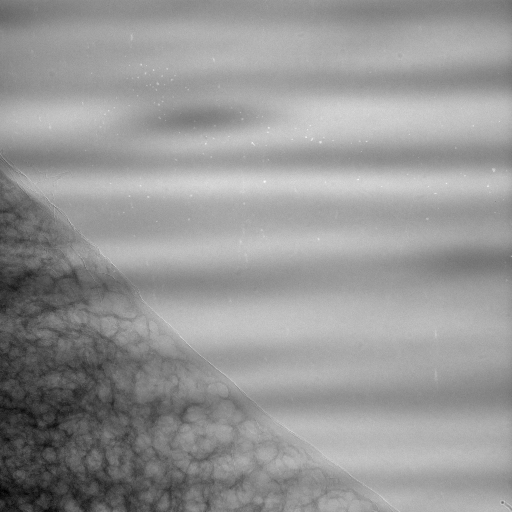
\includegraphics[width=\imsize]{img/merge/R108C10B-s3}}
		\renewcommand{\imsize}{\linewidth}
		\subfloat[Merged and corrected image from the three subscans shown above]{\label{fig:merge-proj}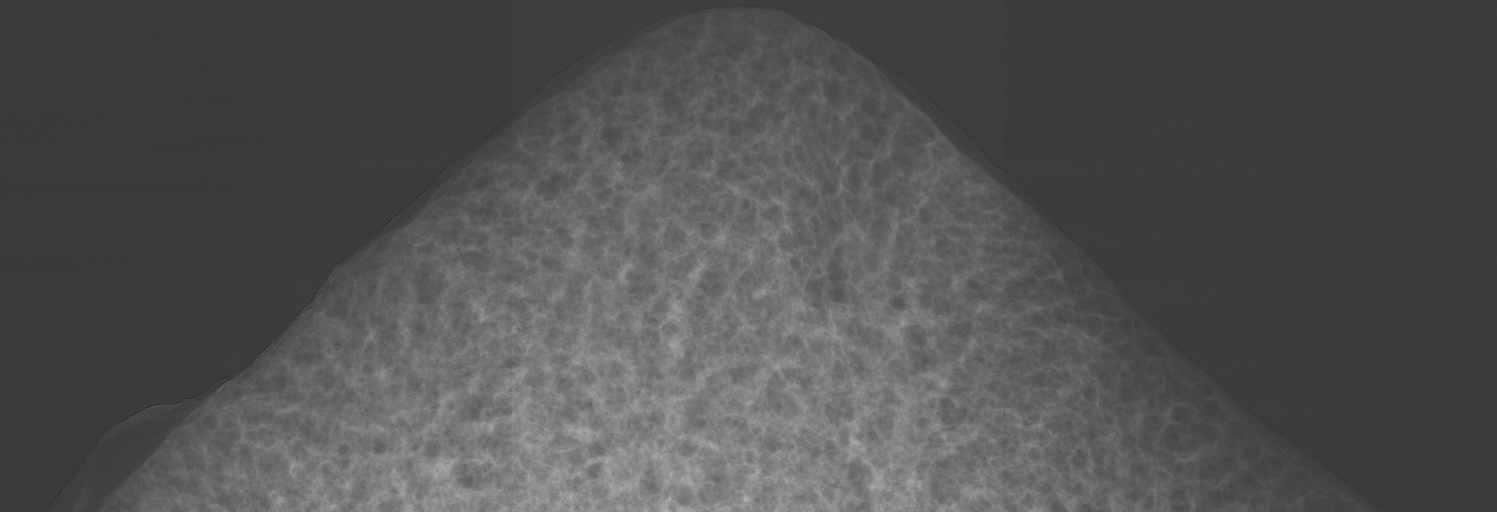
\includegraphics[width=\imsize]{img/merge/R108C10B-merge}}\\
		\subfloat[Reconstructed slice from all projections above]{\label{fig:merge-rec}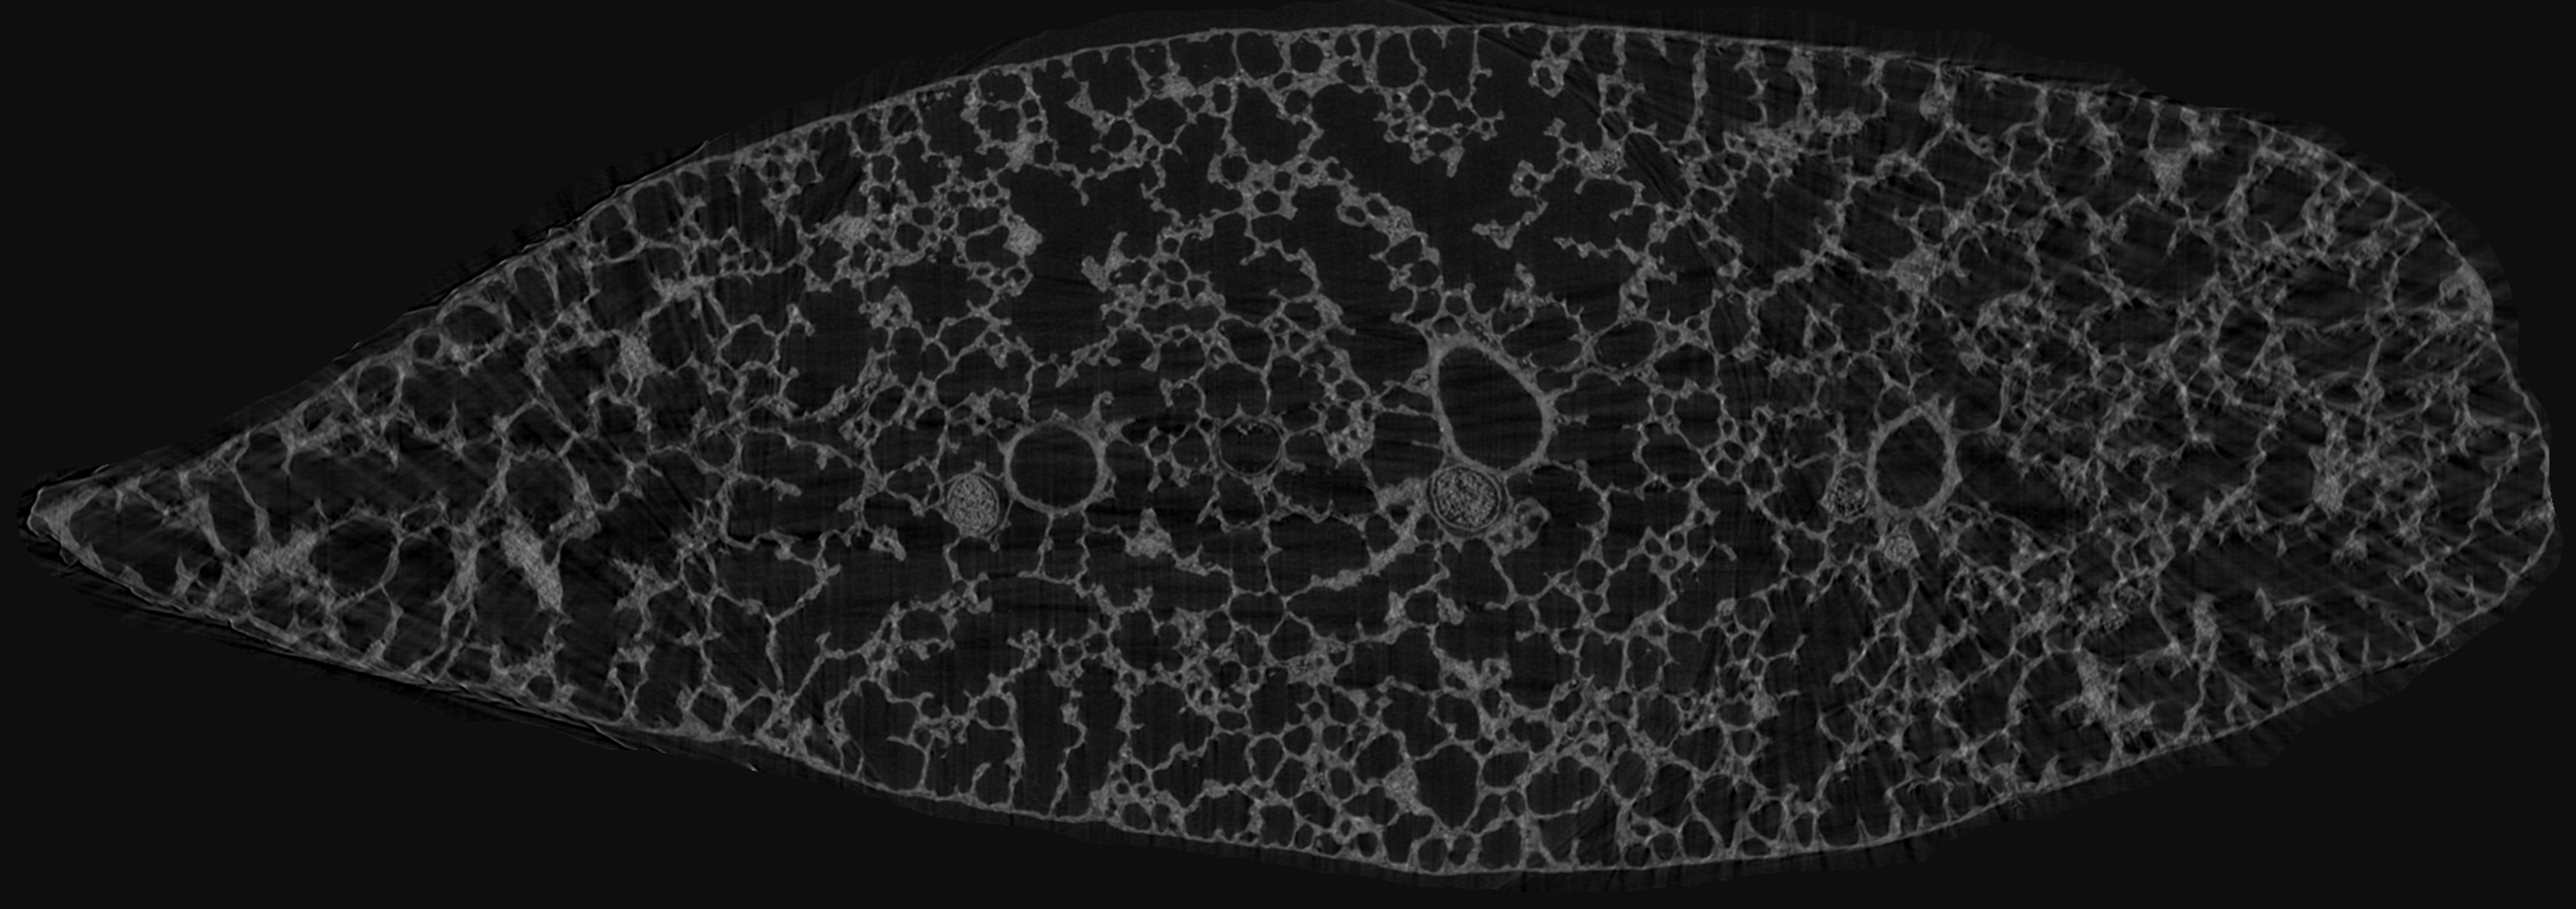
\includegraphics[width=\imsize]{img/merge/R108C10B-merge1016-crop}}\\
	\caption{asdf}
	\label{fig:asdf}
\end{figure}


\section{Publications}
\label{sec:publications}
\subsection{published}
\begin{itemize}
	\item Paper mit Akira~\cite{Tsuda2008}
\end{itemize}

\subsection{submitted}
\begin{itemize}
	\item Proceedings XRM~\cite{Haberthuer2009}
\end{itemize}

\subsection{nds master thesis}
\begin{itemize}
	\item NDS Diplomarbeit~\cite{Haberthuer2008c}
\end{itemize}

\subsection{posters}
\begin{itemize}
	\item Poster @ CIMST~\cite{Haberthuer2008}
	\item Poster @ XRM~\cite{Haberthuer2008b}
\end{itemize}

\subsection{talks}
\begin{itemize}
	\item Tag der Anatomie 2008~\cite{Haberthuer2008a}
	\item NDS-Abschlussweekend~\cite{Haberthuer2008d}
\end{itemize}

\subsection{planned}
\begin{itemize}
	\item wide field scanning
\end{itemize}

\bibliographystyle{unsrtnat}
\bibliography{../../references} % since my LaTeX-files sit in folders like p:\#docs\thisdocument\file.tex and the reference.bib is in p:\#doc

\end{document}